% !TeX root = ..\..\main.tex
\section{ARMA and ARIMA Model}

The first step in building an autoregressive (integrated) moving average (AR(I)MA) model is to determine which process best describes our data. Our process is considered to consist of:

\begin{multicols}{3}
    Autoregressive:
    \begin{equation*}
        \AR{p}: x_t = \sum_{i=1}^p\alpha_ix_{t-i} + \epsilon_t
    \end{equation*}
    \vfill
    \columnbreak
    \noindent Integrated: d is the degree of differencing (the number of times the data have had past values subtracted)
    \vfill
    \columnbreak
    Moving Average:
    \begin{equation*}
        \MA{q}: x_t = \sum_{i=0}^q\beta_i\epsilon_{t-i}
    \end{equation*}
    \vfill
    \columnbreak
\end{multicols}

\subsection{Autoregressive Moving Average Model (ARMA)}

An ARMA model only consist off the $\AR{p}$ and $\MA{q}$ often referred to as $\ARMA{p}{q}$ but is identical to \break$\ARIMA{p}{0}{q}$, expressed mathematically as:

\begin{equation*}
   \ARMA{p}{q} x_t  = \sum_{i=1}^p\alpha_ix_{t-i} + \sum_{i=0}^q\beta_i\epsilon_{t-i}
\end{equation*}
Our problem then is to fit parameters $(p,q)$ that best describe the underlying process of data.

\subsubsection{Finding optimal parameters}

It is possible that our data may have one of the parameters equal 0 meaning that we just an AR or MA process. One way to check this is to calculate both the auto correlation (ACF) and partial auto correlation functions (PACF). Then using the table below we can see if our data satisfies the criteria.
\par\medskip
\begin{center}
    \begin{tabular}{c|c|c|c}
        & AR(p) & MA(q) & ARMA(p,q) \\
        \hline ACF & Tails off & Cuts off after lag $q$ & Tails off \\
        PACF & Cuts off after lag $p$ & Tails off & Tails off \\
    \end{tabular}
\end{center}
\par\medskip
The ACF and PACF functions of our data is shown in \autoref{S2fig:ACFPACF}. Taking a look at the ACF \autoref{S2fig:ACF} we see that we have two peaks at 0.25 and 1.00 (excluding peak at 0). Then looking at the PACF \autoref{S2fig:PACF} we only have one peak at 0.75. This could indicate that we have a $\MA{1}$ process with the peaks at 1.00 and 0.75 being attributed to noise.

\begin{figure}[H]
    \centering
    \begin{subfigure}[b]{\sOneSize\textwidth}
        \centering
        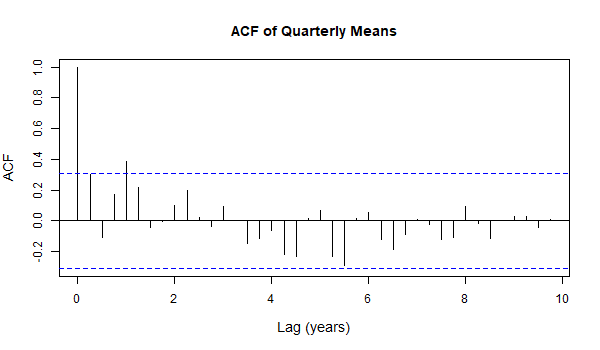
\includegraphics[width=\textwidth]{Sections/ARIMA/Plots/ACF.png}
        \subcaption{Auto correlation function}\label{S2fig:ACF}
    \end{subfigure}
    \begin{subfigure}[b]{\sOneSize\textwidth}
        \centering
        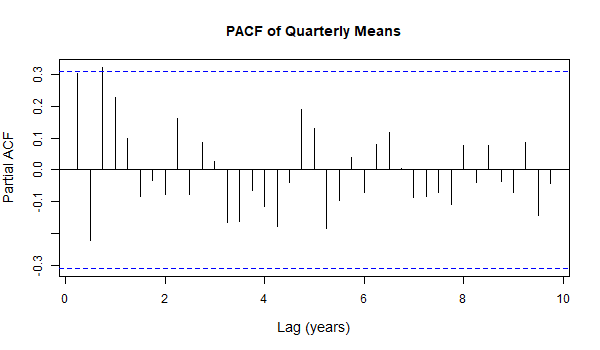
\includegraphics[width=\textwidth]{Sections/ARIMA/Plots/PACF.png}
        \subcaption{Partial auto correlation function}\label{S2fig:PACF}
    \end{subfigure}
\caption{Auto correlation and partial auto correlation functions of our quarterly means data plotted for different lag values in years, with 95\% significance level shown in blue.}
\label{S2fig:ACFPACF}
\end{figure}

However, upon trying values of $(p,q) \in [0,3]\times[0,7]$ and calculating both the AIC and BIC we get the following results:

\begin{table}[H]
    \begin{center}
        \csvautotabular{S2Tab1.csv}
    \end{center}
    \caption{Sum of AIC and BIC for different $(p,q)$ pairs. For $q > 7$ or $p > 3$ the parameter pair approach the end of the stationarity region.}
    \label{S2:tab_sum}
\end{table}

\begin{itemize}
    \item \input{Sections/ARIMA/Outputs/min1.txt}
    \item \input{Sections/ARIMA/Outputs/min2.txt}
    \item \input{Sections/ARIMA/Outputs/min3.txt}
\end{itemize}

We then conclude that the optimal parameters for our ARMA model are $\ARMA{0}{1}$.